\documentclass{standalone}

\RequirePackage[T1]{fontenc} \RequirePackage[tt=false, type1=true]{libertine}
\RequirePackage[varqu]{zi4} \RequirePackage[libertine]{newtxmath}

\pdfoutput=1

\usepackage{amsfonts}
\usepackage{tikz}
\usetikzlibrary{arrows.meta}

\begin{document}


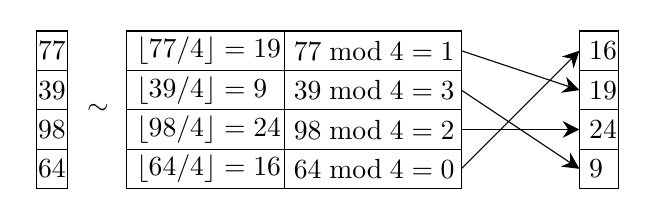
\begin{tikzpicture}

\draw(-2,0)   node[right] {$64$};
\draw(-2,0.5) node[right] {$98$};
\draw(-2,1)   node[right] {$39$};
\draw(-2,1.5) node[right] {$77$};

\draw (-1.9,1.75) rectangle (-1.5,-0.25);
\draw (-1.9,1.25) rectangle (-1.5,0.25);
\draw (-1.9,0.75) -- (-1.5,0.75);

\draw(-1.375,0.75) node[right] {$\sim$};

\draw(-0.75,0)   node[right] {$\lfloor 64/4 \rfloor = 16$};
\draw(-0.75,0.5) node[right] {$\lfloor 98/4 \rfloor = 24$};
\draw(-0.75,1)   node[right] {$\lfloor 39/4 \rfloor = 9$};
\draw(-0.75,1.5) node[right] {$\lfloor 77/4 \rfloor = 19$};

\draw(1.25,0)   node[right] {$64 \bmod 4 = 0$};
\draw(1.25,0.5) node[right] {$98 \bmod 4 = 2$};
\draw(1.25,1)   node[right] {$39 \bmod 4 = 3$};
\draw(1.25,1.5) node[right] {$77 \bmod 4 = 1$};

\draw (-0.75,1.75) rectangle (3.5,-0.25);
\draw (-0.75,1.25) rectangle (3.5,0.25);
\draw (-0.75,0.75) -- (3.5,0.75);
\draw (1.25,-0.25) -- (1.25,1.75);

\draw(5,0)   node[right] {$9$};
\draw(5,0.5) node[right] {$24$};
\draw(5,1)   node[right] {$19$};
\draw(5,1.5) node[right] {$16$};

\draw (5,1.75) rectangle (5.5,-0.25);
\draw (5,1.25) rectangle (5.5,0.25);
\draw (5,0.75) -- (5.5,0.75);

\draw [-{Stealth[length=6, width=6]}] (3.5,1.5) -- (5,1);
\draw [-{Stealth[length=6, width=6]}] (3.5,1)   -- (5,0);
\draw [-{Stealth[length=6, width=6]}] (3.5,0.5) -- (5,0.5);
\draw [-{Stealth[length=6, width=6]}] (3.5,0)   -- (5,1.5);

\end{tikzpicture}

\end{document}
